\documentclass[12pt]{article}

\usepackage[backend=biber]{biblatex}
\usepackage[margin=1in]{geometry}
\usepackage[utf8]{inputenc}
\usepackage{setspace}
\usepackage{amsmath}
\usepackage{amssymb}
\usepackage{mathtools}
\usepackage{esint}
\usepackage{titlesec}
\usepackage{graphicx}
\usepackage{wrapfig}
\usepackage{blindtext}
\usepackage{fancyhdr}
\usepackage{caption}
\usepackage{subcaption}
\usepackage{wallpaper}

\ThisLRCornerWallPaper{1.2}{./figures/bgimage.png}

\addbibresource{/home/krttd/documents/UAH.bib}

\doublespacing

\pagestyle{fancy}
\lhead{}
\chead{}
\cfoot{}
\rhead{Dodson \thepage}

\renewcommand*{\bibfont}{\normalsize}

%\titleformat{\section}
%{\large}{}{0em}{}[\titlerule]

%\titleformat{\subsection}
%{\large}{}{0em}{}


\begin{document}

\thispagestyle{empty}
\vspace*{5em}
\begin{center}\Huge\sc
  SPoRT BLOG
\end{center}

\begin{center} \Huge
  Software Design and Philosophy Report
\end{center}

\vspace*{3em}
\begin{center} \Large
  Mitchell T. Dodson
\end{center}

\vfill

\begin{center} \Large
  Eh 301 Term Project

  April 27, 2020
\end{center}

\vspace*{3em}
\newpage

\tableofcontents
\newpage

\begin{figure}[h]
  \centering
  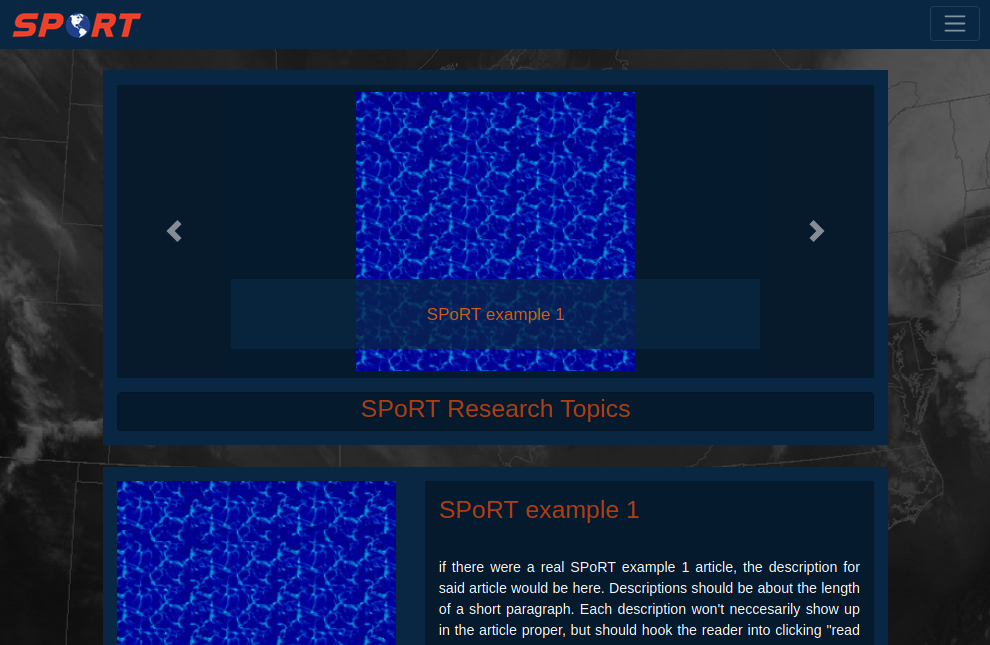
\includegraphics[width=.66\textwidth]{./figures/website-ss.png}
  \caption{Front Page Concept}
  \label{front page} %(to reference in the future text)
\end{figure}

\section{Introduction}

Development of the SPoRT blog began in January of 2020. As of April 2020, the blog is still an ongoing project led by UAH undergraduate students and overseen by NASA-MSFC civil servants. The web blog is projected to be completed and open to the public around June 2020, at which time it will be hosted at \texttt{https://weather.msfc.nasa.gov}.

This document provides a detailed outline of the structure of the SPoRT Blog software suite, describes the design principles and philosophies that informed choices made by its developers, and gives exhaustive API information for each software module. These discussions are divided into three topics: the blog front-end, back-end, and publishing system, which reflects the discrete structure of the software itself.

The SPoRT blog software suite will never be fully publicly available, however this report \textit{will} be open to the public. For security reasons, some details including internal network information, fully-qualified directory paths, and input form sanitization methods must be omitted from this document.

\newpage
\section{Background}

\subsection{What is SPoRT?}

\begin{wrapfigure}{r}{.35\textwidth}
  \centering
  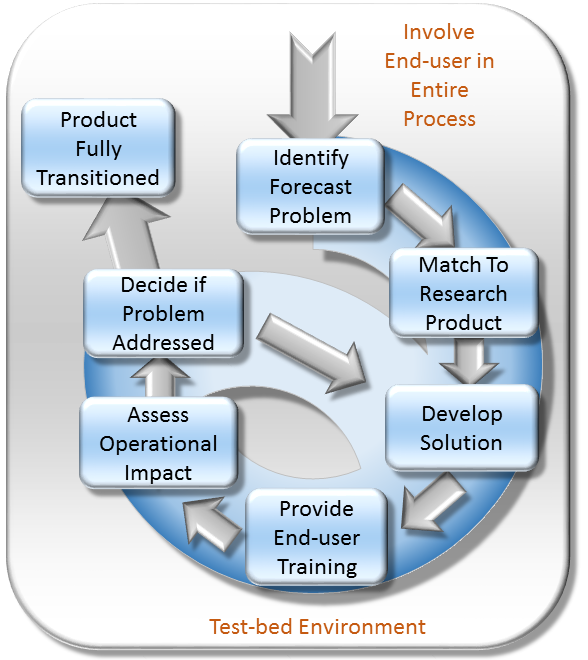
\includegraphics[width=\linewidth]{./figures/sport-process.png}
  \caption{the SPoRT process \cite{SPoRT18b}}
  \label{partners} %(to reference in the future text)
\end{wrapfigure}

\textit{Short-Term Prediction, Research, and Transition} (SPoRT) is a long-term atmospheric science project funded by NASA's Marshall Space Flight Center (NASA-MSFC) and the National Oceanic and Atmospheric Administration (NOAA) in collaboration with the UAH Earth Systems Science Department (UAH-ESS). SPoRT's main focus is to collect and process rapidly incoming satellite and radar imagery, which assists local and international forecasters and researchers. SPoRT publishes all its research and real-time imagery publicly on their website \cite{SPoRT_RTD20} along with detailed descriptions of the products, so SPoRT's internal forecasting expertise can be fully accessed by citizen scientists and anyone interested in receiving less watered-down weather information.

\subsection{What is the SPoRT Blog?}

Although SPoRT is officially a public-facing project, the organization is usually viewed as an intermediate component of the atmospheric science research and forecasting process. SPoRT leadership believes the project has a lot to offer the public, so an initiative to develop a locally-hosted blog was created in order to facilitate more direct lines of communication between researchers, forecasters, software developers, and anyone in the public.

\newpage
Articles will be tailored to a high school reading level and will spotlight graduate students and their research, showcase interesting results and conclusions from civil servants' projects, announce new long-term projects and data sources, and reflect on major local weather events. Find examples of articles in SPoRT's current newsletter site \cite{sportnewsletter20}, which the blog will replace.

\section{Who is this document for?}

This software design report is oriented towards software developers, particularly system administrators and developers working for NASA-SPoRT responsible for maintenance of the SPoRT blog. Furthermore, since the SPoRT blog is heavily modularized, SPoRT developers will find this document useful for reference when forking the blog software to be used in other programs. In addition to being a procedural outline of the blog software intended for technical reference, this document serves as a sort of treatise on many elements of the SPoRT software design philosophy (naming schemes and API structure, for instance). For this reason, software developers in general -- especially those responsible for system maintenance, small-scale databasing, and dynamic webpage design -- may appreciate this software design report as a source of inspiration for their own projects.

\newpage
\section{SPoRT blog front-end}
\label{frontend}

The SPoRT blog landing page was designed with the Bootstrap4 framework: a 'mobile-first' framework which provides useful utilities for specifying geometric properties of the webpage, creating navigation bars and 'carousel' links, and setting breakpoints.

When developing the front-end design of the SPoRT blog webpage, usability, extensibility, and intuitive layout were the foremost goals. Users should be able to quickly sort the database of articles by pre-assigned article topics, and should also be able to search the database for specific keywords within articles.

\subsection{Modular layout}
\label{modules}

\begin{figure}[h]
  \centering
  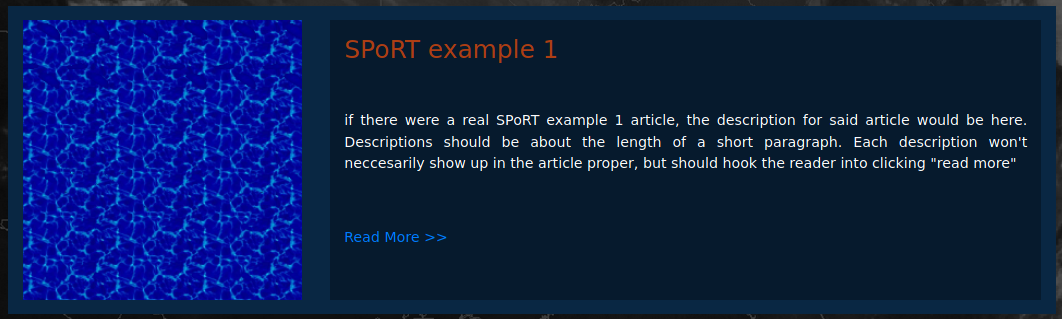
\includegraphics[width=.66\linewidth]{./figures/module.png}
  \caption{Article module format}
  \label{module example} %(to reference in the future text)
\end{figure}

 The blog in principle is a fairly simple and uniform construct: each article is a collection of formatted text and images with a title, an upload date, and a series of topics (see section \ref{publishing} for topic assignment), and the landing page itself is just a collection of articles, as well as tools for sorting and filtering those articles. Because of these properties, we decided to abstract each individual article as a structure containing a 256x256 thumbnail image, a title, a short description, a list of relevant topics, and a link mapping the structure to the full article. For the remainder of this document, these structures will be refered to as "modules".

 The concept of a module is incredibly useful for database sorting and organization as well as the landing page's browser efficiency. It's clearly unreasonble to write articles directly to the html document associated with the landing page; if articles were presented statically like this, it would be impossible for users to sort articles. Furthermore, static articles would require the entire webpage, along with all the uploaded articles, to be loaded any time the website is visited; this would substantially tax the webserver, and users with slow internet connections would have a \textit{very} difficult time viewing anything. Using modules, AJAX requests can wait until users scroll down to fill in the necessary information; Section \ref{backend} and Figure \ref{module creation} detail this process.

\begin{wrapfigure}{r}{0.25\textwidth}
  \begin{center}
    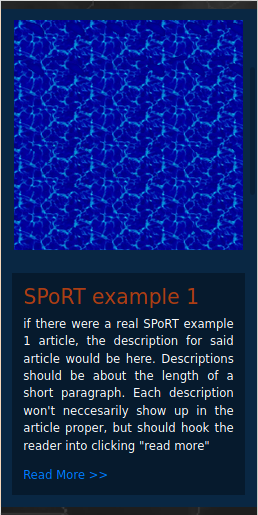
\includegraphics[width=0.23\textwidth]{./figures/phone-module.png}
  \caption{Module format on mobile browser}
  \label{phone module}
  \end{center}
\end{wrapfigure}

 As far as front-end design is concerned, the module system allows for 'infinite' scrolling as well as lazy loading; when users visit the landing page, the only modules that load are the ones that are \textit{on their screen} at any point in time. Cosmetically, modules follow the format of the example seen in Figure \ref{module example}; users will see a descriptive thumbnail image chosen by the publisher of the article, as well as the title and a short description of the article's contents. Modules are clickable via stretched links, and will load and display the full article by Common Gateway Interface (CGI) fetching upon link activation.

When viewed by mobile device browsers or browsers with very narrow aspect ratios, modules will change their geometry and stack vertically, as seen in Figure 4. This doesn't affect any of the landing page's or modules' features.

\newpage

\subsection{Sorting tools}
\label{landing page}

\begin{figure}[h]
  \centering
  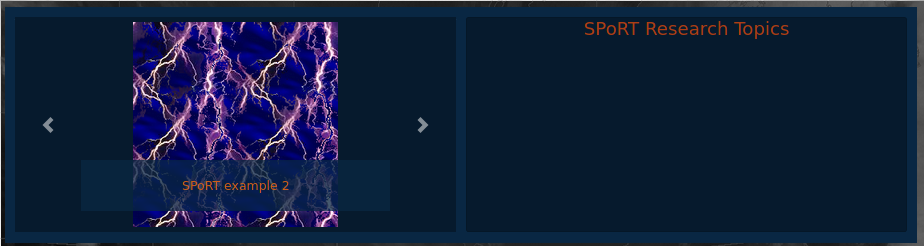
\includegraphics[width=.66\linewidth]{./figures/display.png}
  \caption{Landing page display banner}
  \label{display} %(to reference in the future text)
\end{figure}

Users will have the option to sort by article upload month/year, user-provided keyword, or by a series of preassigned topics designated by each article's publisher. Unfortunately, graphical examples of these utilities cannot be provided at the time of writing since fetching topic categories requires the live database to be actively hosted by the web server. When the database and website \textit{are} finally live, topics will include

\begin{itemize}
  \item{\textbf{Graduate spotlights}: profiles of SPoRT graduate students and their research.}
  \item{\textbf{SPoRT News}: major research updates and project announcements.}
  \item{\textbf{SPoRT scientist spotlights}: profiles of SPoRT civil servants and contracting scientists and descriptions of their projects.}
  \item{\textbf{Project updates}: research updates from long-term projects. Currently there are 33 actively-publishing projects under SPoRT, each of which will have its own category. See the current SPoRT newsletter \cite{sportnewsletter20} for a full list.}
  \item{\textbf{Outreach}: Announcements for SPoRT-organized events and other outreach programs.}
\end{itemize}

Article publishers will have the option to assign multiple topics to any article, or to add new topics if necessary. This way, when a  user selects a specific topic and modifies their search in any way (such as constraining the upload date or using keywords), the only modules that will be loaded and displayed for them will be those which belong to one or more of the relevant topics and which fulfill their constraints.

\subsection{Accessibility}
\label{accessibility}

\begin{figure}
\centering
\begin{subfigure}{.5\textwidth}
  \centering
  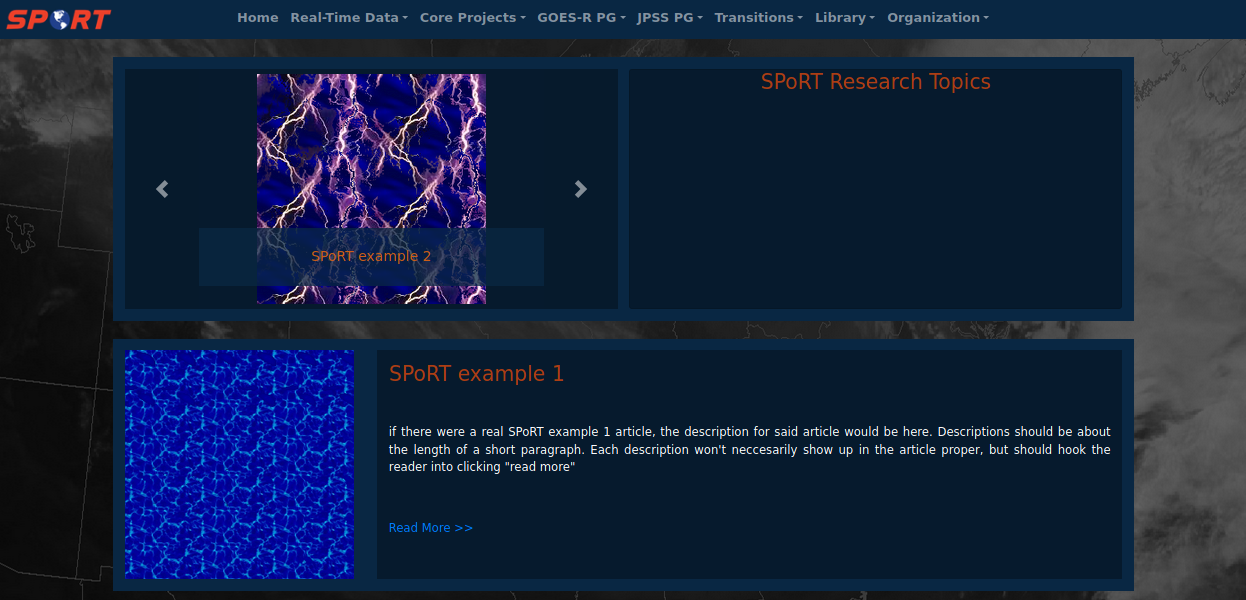
\includegraphics[width=.98\linewidth]{./figures/acc-unaffected}
  \caption{unaffected}
  \label{acc-unaffected} %(to reference in the future text)
\end{subfigure}%
\begin{subfigure}{.5\textwidth}
  \centering
  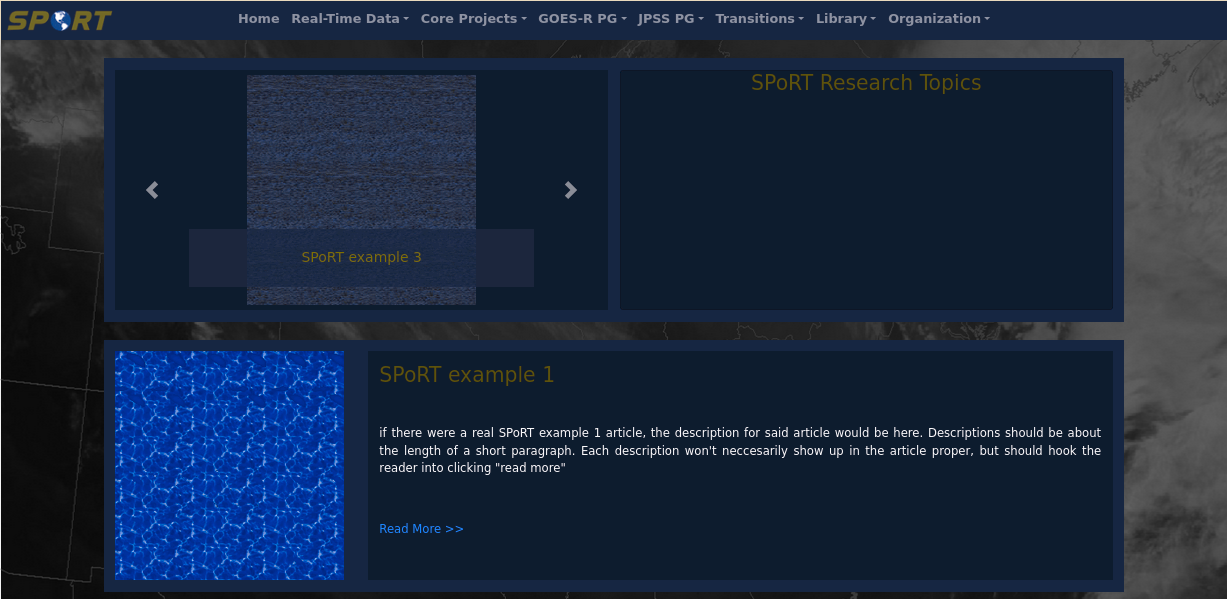
\includegraphics[width=.98\linewidth]{./figures/acc-protanomaly}
  \caption{protanomaly}
  \label{acc-protanomaly} %(to reference in the future text)
\end{subfigure}
\end{figure}

\begin{figure}
\centering
\begin{subfigure}{.5\textwidth}
  \centering
  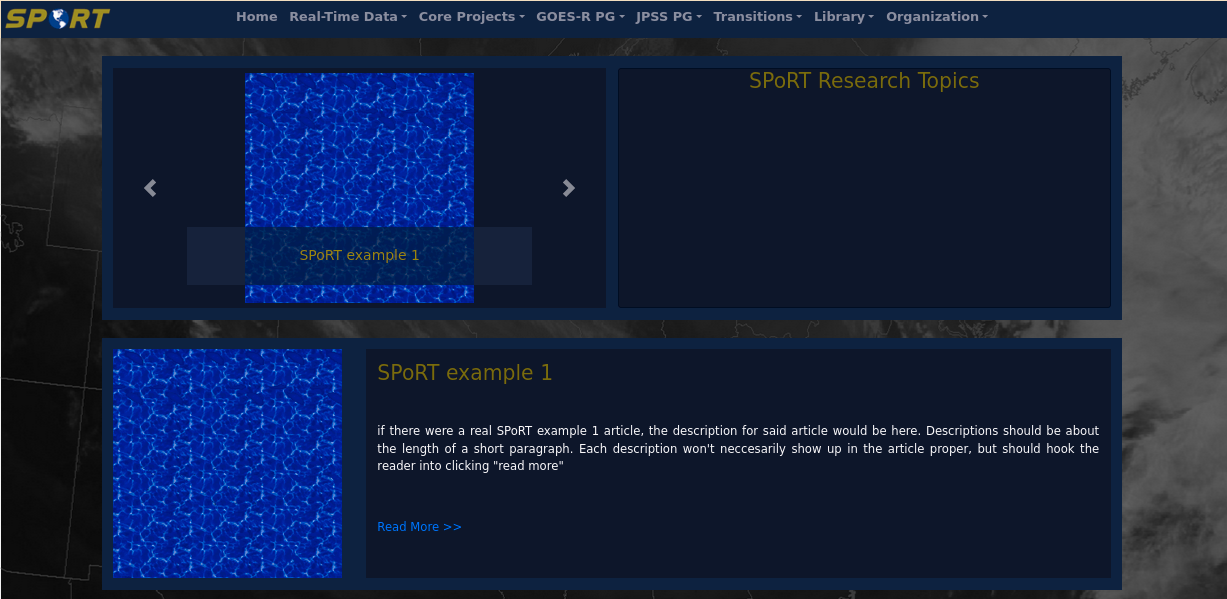
\includegraphics[width=.98\linewidth]{./figures/acc-deuteranomaly}
  \caption{deuteranomaly}
  \label{acc-deuteranomaly} %(to reference in the future text)
\end{subfigure}%
\begin{subfigure}{.5\textwidth}
  \centering
  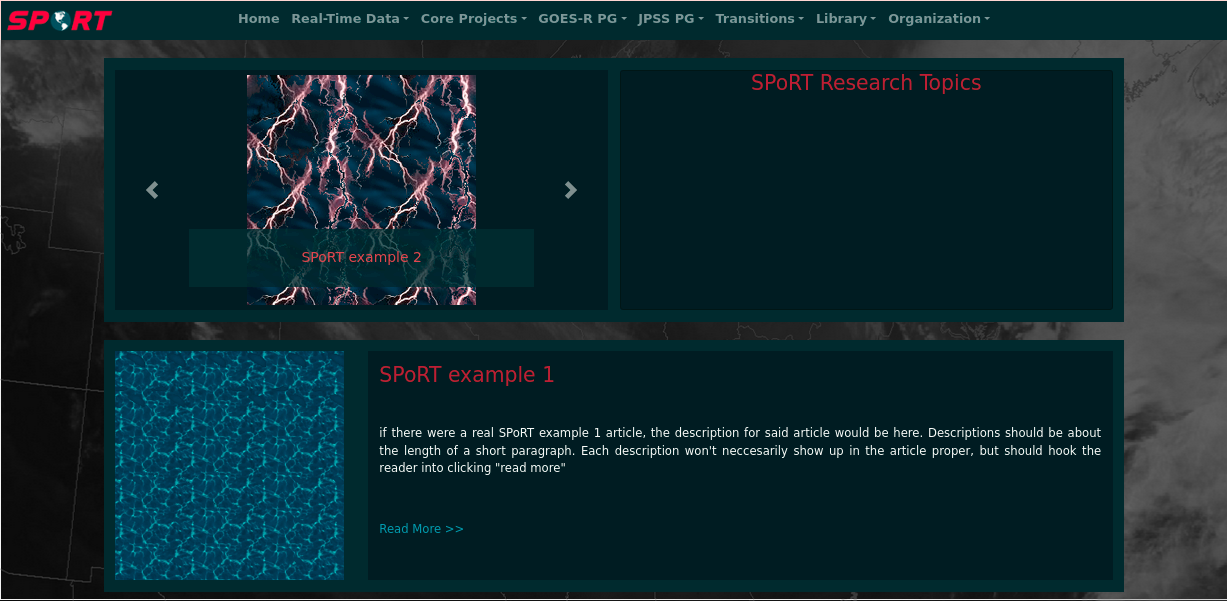
\includegraphics[width=.98\linewidth]{./figures/acc-tritanomaly}
  \caption{tritanomaly}
  \label{acc-tritanomaly} %(to reference in the future text)
\end{subfigure}
\caption{Colorblindness accessability test results (using firefox utility \cite{lgcb20})}
\label{colorblindness}
\end{figure}

Website accessibility was one of the most important factors influencing design choices. In order to accommodate users affected by colorblindness, we used a firefox browser add-on \cite{lgcb20} which simulates 3 common types of color vision deficiency (Figure \ref{colorblindness}). This extension allowed us to experiment with several color scheme choices to find combinations that are sufficient for colorblind users, and fit the SPoRT brand standards. We ultimately chose a navy/orange combination that contrasted well under each of the simulated conditions.

Additionally, one of the main reasons developers chose the Bootstrap4 framework is the library's excellent compatibility with text-to-speech and webpage magnification software. The vertical layout of the webpage combined with the relative brevity of individual module descriptions means text-to-speech software that parses out specific html elements (such as headers or list items) will do so concisely and consistently. Furthermore, the organization of elements will keep their logical order (this is untrue for webpages that rely on navigation and topic utilities located in side bars). Moreover, the ``stackability'' of containers such as modules and the display banner (see Figure \ref{phone module}) allow the webpage to magnify seamlessly without losing its geometric properties.

\newpage
\section{SPoRT blog back-end}
\label{backend}

One of the biggest challenges faced by developers of the SPoRT blog has been creating a well-organized databasing system for efficiently and securely delivering modules to visitors of the blog.

\noindent
In order to be effective, the blog backend must:
\begin{itemize}
  \item{operate automatically such that manual database intervention isn't typically required.}
  \item{store modules and articles in human-readable formats so developers can make live edits.}
  \item{retrieve data very quickly when modules and articles are requested by a user.}
  \item{avoid reliance on external databasing software such as mongoDB or SQL (for security).}
  \item{maintain compliance with the Freedom of Information Act (FOIA). \cite{foia20}}
\end{itemize}

\subsection{Module creation}
\label{module creation}

As briefly discussed in Section \ref{modules}, the only article modules that will be loaded for a user at any point in time are those which are actively being displayed for the user. The blog backend facilitates this principle by `filling in' initially-empty div environments on the landing page based on the search constraints imposed by the user. This is accomplished by using the get-modules CGI script, which collects user-provided constraints and translates them into a list of local addresses. Once the CGI script returns the list of local addresses (as javascript array of strings), the landing page iterates through the list, making an ajax request for the module located at each address, and assigns each subsequent module to one and only one empty div environment.

\newpage

\begin{figure}[h]
  \centering
  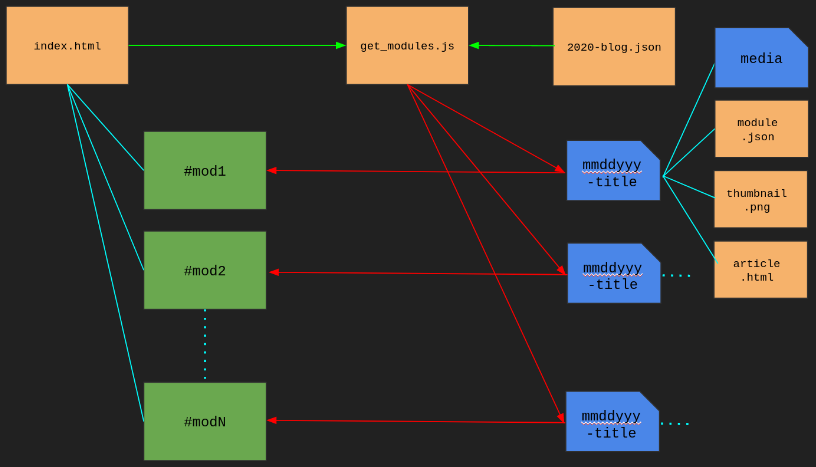
\includegraphics[width=.8\linewidth]{./figures/module-fill.png}
  \caption{Module creation process (on AJAX call)}
  \label{module creation} %(to reference in the future text)
\end{figure}

When a user applies a constraint, for example by clicking on the check-box form for the NUCAPS topic and constraining the dates to 2018-2019, the form modifies the URL and subsequently the request made to the server. If no constraints are applied, the user's URL might look like this:

\begin{center}\tt\footnotesize
  https://weather.msfc.nasa.gov/sport\_blog/
\end{center}

\noindent
however when the user apples the constraint, the URL is extended by the appropriate parameters. Using the check-box example from above, the user's URL might look like this:

\begin{center}\tt\footnotesize
  https://weather.msfc.nasa.gov/sport\_blog/cgi-bin/get-modules?topic=nucaps\&yi=2018\&yf=2019
\end{center}

Where \texttt{get-modules} is the CGI script and \texttt{topic}, \texttt{yi}, and \texttt{yf} are parameters corresponding to the user's selections for the topic, the initial year, and the final year respectively.

In a practical sense, the 'addresses' retrieved by the get-modules script are simply paths to the unique subdirectory of every module that abides by the user's parameters (i.e. date range, topic, keywords). See Figure \ref{module creation} for a diagram of the entire process, and Figure \ref{directories} for a visualization of the database directory.

\newpage
\subsection{directory/database structure}
\label{database}

\begin{figure}[h]
  \centering
  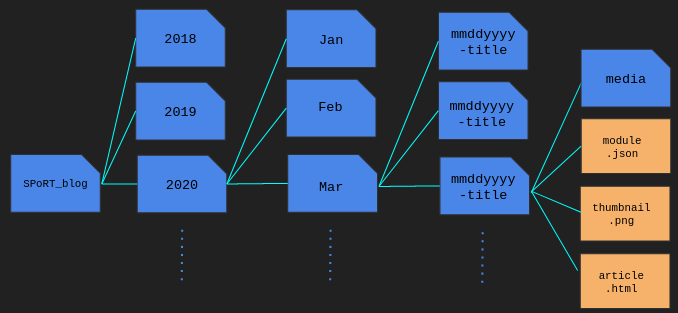
\includegraphics[width=.8\linewidth]{./figures/directories.png}
  \caption{SPoRT Blog Directory Structure}
  \label{directories} %(to reference in the future text)
\end{figure}

As mentioned at the beginning of Section \ref{backend}, the databasing system for storing articles  and their corresponding modules must remain well-organized and human-readable in order to facilitate live-editing of articles that are already published, and to allow for straightforward aggregation of articles and article information in the event of a FOIA request. Additionally, the system must not rely on software such as mongoDB or SQL; since the database is a public-facing utility, 3rd party databasing software poses represents a potential vulnerability.

In order to comply with these requirements, the SPoRT database stores blog publications in a chronologically-organized hierarchical directory tree and collects article information in a static json document specific to the year of publication. The json document is a complete index of articles published that year, and is responsible for storing the each article's title, location, publication date, and topics. This document is updated any time an article is published (Figure \ref{publishing process}).

Articles are held in unique directories adhering to a \texttt{MMDDYYY-title-of-article}  naming scheme. This naming scheme allows sysadmins and developers to quickly find an article corresponding to a specific date (since directory listings are typically organized by numerical value and alphabetical order), or to skim articles by title. Each subdirectory contains the article iteslf titled \texttt{article.html}, the module thumbnail picture titled \texttt{thumbnail.png}, and the module information titled \texttt{module.json}, along with a subdirectory titled \texttt{media} which contains any other images or videos used in the article. The names of files within each article's directory are always consistent with the above standard, so as long as the landing page has the fully-qualified path to the article directory, each of the files contained therein can be easily retrieved. See figure \ref{directories} for a graphical representation of this system.

Unfortunately this report cannot provide details on the more high-level structure of the database, nor can it specifically detail the particular ways the web server queries the database since such information could potentially be compromising to security.

\subsection{FOIA compliance}
\label{foia compliance}

The Freedom of Information Act (FOIA) provides that any individual has the right to request the records and information of federal agencies including NASA \cite{foia20}. In order to comply by FOIA's statutes, SPoRT must be able to produce an organized collection of all records with short notice. In the case of the SPoRT blog, information that SPoRT is obligated to produce includes all articles published during the time frame stipulated by the request, as well as the date/time of publishing/modification of every article.

The chronological organization of the database as covered in Section \ref{database} makes providing the articles themselves a fairly straightforward task. In order to report the upload and modification time of each article, the year-specific persistent json document mentioned in section \ref{database} will also automatically record the relevant information as shown under the `Web Server' section of Figure \ref{publishing process}.

\newpage
\section{SPoRT blog publishing system}
\label{publishing}

\subsection{Interviews with publishing researchers}
\label{interviews}

In order to better understand the amount of experience SPoRT research scientists generally have with command-line utilities, anonymous interviews were conducted with 3 of the scientists working on 3 different projects. The following questions were posed to the interviewees, and their responses are reported  in Figure \ref{results}.

\begin{enumerate}
  \item{How familiar are you with using command-line interfaces (CLIs)?}
  \item{What specific command-line programs, if any, do you regularly use?}
  \item{How do you usually get information about CLI usage?}
\end{enumerate}

\vspace{2em}
\begin{figure}[h]
  \centering
  \begin{tabular}{l | l | l | l }
     & \textbf{Q1} & \textbf{Q2} & \textbf{Q3} \\\hline
    \textbf{Interviewee 1} & very; use daily & vim, ssh, stat, etc.  & man pages, help flags, internal docs \\
    \textbf{Interviewee 2} & somewhat & ssh, cat, python & internet, help flags \\
    \textbf{Interviewee 3} & proficient & ssh, perl, feh, ffmpeg & man pages, help flags, internet\\
  \end{tabular}
  \caption{Interview responses}
  \label{results}
\end{figure}

From the responses, we determined that making a simple command-line client would be reasonable, especially when accompanied with a guide \cite{dodson20} providing detailed instructions on how to use the CLI and accompanying options. We know that all researchers who will be publishing are at least familiar with SSH since all research at SPoRT is conducted primarily on remote machines that the scientists must SSH into. With this information, the development team decided to distribute publication software exclusively to SPoRT-run research and production machines, which makes version control vastly more simple than if software needed to distributed to individuals' work machines as well.

\subsection{Publishing command-line interface}
\label{cli interface}

The CLI used for publishing is a python-based package distributed to each SPoRT production/research machine via anaconda environment version control. This CLI is responsible for prompting the user for all the necessary information about an article, such as a title, description, thumbnail, and the article itself. In practice, the interface is a series of 2 commands, the first of which, \texttt{blogprepare}, accepts the article itself from the user and provides a json document acting as a form for the user to fill out. After filling out the json document, the user runs the second command, \texttt{blogpublish}, which accepts the json document and initiates the rest of the publishing process as discussed in Section \ref{remote machine publishing}.

\begin{figure}[h]
  \centering
  \begin{tabular}{l | p{8cm}}
  \textbf{modifier} & \textbf{purpose} \\\hline
  \texttt{--keep-article} & save the original article and thumbnail image to the current machine. \\\hline
  \texttt{--keep-module-json} & keep the json form for setting title/description. \\\hline
  \texttt{-i} \textit{/path/to/image} & specify the path to the article thumbnail image. If the image is not a 1x1 aspect ratio, it will be automatically cropped. \\
  \end{tabular}
  \caption{Publishing command options}
  \label{cli opt}
\end{figure}

At the time of writing, the command modifiers found in Figure \ref{cli opt} allow publishers to specify the thumbnail image and retain the json form or article after the publishing process has finished. Users can pass these options to either of the commands. If different images are provided to each of the commands, the user will be asked to choose which thumbnail to use before the article package gets transferred to the web server.

In order to make publishing as simple as possible for the researchers, even filling out the json form is presented as optional. For example, if no description, image or title is provided, the interface will attempt to establish a reasonable title, description, and thumbnail image by parsing the article itself. Once the default features have been selected, the user will be asked to confirm that the automatically-selected fields are sufficient prior to publishing. Moreover, even if no image can be found, the client will ask the user if they wish to select one of the pre-made default article thumbnails, at which point they can choose from the defaults or decide to upload their own.

The module format requires that thumbnail images always adhere to a 256x256 pixel resolution in order to reduce module loading times and keep module geometry consistent. If the publishing scientist provides a higher-resolution image, the client will automatically copy the user-provided image and reduce the resolution of the copy using cubic interpolation provided by the imagemagick toolkit. Likewise, if the provided image has an aspect ratio other than 1x1, the client will copy and crop the image using imagemagick. In either case, the copied and modified image is presented to the user, at which point the user can choose to either accept the automatically-edited image or upload a new image.

\begin{figure}[h]
  \centering
  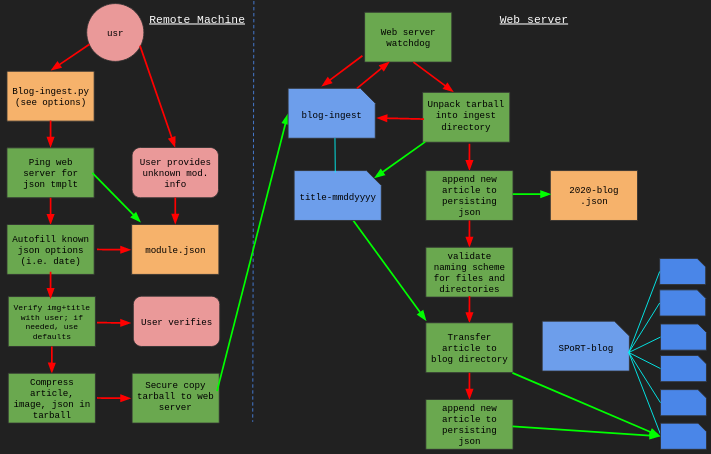
\includegraphics[width=.8\linewidth]{./figures/publishing.png}
  \caption{Blog publishing process}
  \label{publishing process} %(to reference in the future text)
\end{figure}


\subsection{Transferring from remote machines}
\label{remote machine publishing}

Although the packaging and transfer components of the publishing library are housed in a different software module than the CLI client, they are distributed to the SPoRT machines in the same anaconda environment so that version control is identical. By distributing these modules together, we guarantee that differences in the modules' `age' will never be responsible for a conflict in their interaction.

The software component of the publishing library responsible for formatting, packaging, and transferring articles is instantiated by the CLI client as soon as the client is finished prompting the user for all needed information. Upon instantiation this module renames the thumbnail image, json info file, article document, and media files according to a \texttt{MMDYYY-article-title} format. By temporarily renaming files in this manner, name collisions in the web server ingest directory can be prevented.

After renaming the article files, the transfer module packages and compresses them in a tar archive so that the entire directory can be transferred in one action. Since all of the SPoRT research and production machines that can publish to the blog are necessarily members of the SPoRT intranet, the module simply sends the newly-created tar archive to a registered directory (blog-ingest in Figure \ref{publishing process}) in the web server via Secure File Transfer Protocol (sftp).

\subsection{Web server article ingesting}
\label{web server publishing}

As discussed in Section \ref{database}, one of the goals the development team had while designing the article database was to avoid the need for any manual intervention. In order to automate the process of article registration and database organization, the appearance of an article in the ingest directory triggers an INOTIFY event. When this INOTIFY event associated with the ingest directory occurs, a watchdog process recognizes the event and instantiates the web server's article ingest module.

When the ingest module is called by the watchdog it immediately decompresses the new article into a subdirectory of the ingest directory following the same \texttt{mmddyyy-article-title} naming format used by the article elements contained therein. From this stage onward, the full identity of the article can be established by parsing the name of the directory that holds it. At this point, the module knows everything about the article including its title, publishing date and time, and assigned topic, and updates the persistent json (see \texttt{2020-blog.json} in Figure \ref{publishing process}) with this information. To be clear, this json document is the same file used by the web server for module lookups and for aggregating publishing info in case of a FOIA request (Sections \ref{module creation}, \ref{foia compliance}).

Next, the module renames each element of the article according to the naming scheme specified in Figure \ref{directories}. By making all article file names identical, the web server only needs to recieve the name of the directory that holds them in order to have full access to each component of the article. Once the naming is consistent with the format anticipated by the database, the module simply parses the article month and year and transfers the entire article directory to the appropriate location in the web server's database. At last, the article is `live,' and will be immediately accessible worldwide through the blog website.

\section{Moving forward with the SPoRT blog}

Although the SPoRT blog is expected to be fully operational by June of 2020, development of useful blog features and utilities will continue indefinitely. The development team looks forward to adding new features such as a GUI image cropping system for the publishing client or a commenting system / discussion board for the website. Additionally, some currently-implemented features of the blog suite stand to be improved in the future -- for example a syntax matching system could substantially improve the quality of the search feature. If you have any comments or suggestions regarding the SPoRT blog, please feel free to email them to \texttt{mitchell.t.dodson@nasa.gov} or contact any member of the SPoRT project leadership.

\nocite{Brooke18}
\nocite{Melbourne15}
\nocite{Ceta20}
\nocite{blender19}

\newpage
\printbibliography
\end{document}
